\documentclass[12pt]{article}
\usepackage{textcomp}
\usepackage{cmap}				    	% поиск в PDF
\usepackage{mathtext} 	           
\usepackage[T2A]{fontenc}			% кодировка
\usepackage[utf8]{inputenc}			% кодировка исходного текста
\usepackage[english]{babel}
\usepackage[colorlinks=true,urlcolor=darkgray,citecolor=darkgray,linkcolor=darkgray,bookmarks=true]{hyperref}
% \usepackage{ccaption}
\usepackage{authblk}
\usepackage{indentfirst}
% \usepackage{float} 
\usepackage{amsmath}
\usepackage{apacite}
\usepackage{natbib}
\usepackage{graphicx}
\usepackage{comment}
\usepackage{amsfonts}
\usepackage{bm}
\usepackage{amssymb}
\usepackage{amsthm}
\usepackage{mathtools}
\usepackage{upgreek} % AMS
\usepackage{marvosym}
\usepackage{threeparttable}
\usepackage{etoolbox}
\usepackage{cmap}	
\usepackage{multirow}
\usepackage{fullpage} 
\usepackage{geometry}
\geometry{
 a4paper,
 total={210mm,297mm},
 left=20mm,
 right=20mm,
 top=20mm,
 bottom=20mm,
 }
\usepackage{url}
\usepackage{pgfplots}
\usepackage{caption}
\usepackage{longtable}
\usepackage{multirow}
\usepackage{booktabs}
\usepackage{makecell}

\usepackage{pgf}
\usepackage{tikz}
\pgfplotsset{compat=1.15}
\usepackage{mathrsfs}
\usepackage{tikz} 
\usepackage{pgfplots}
\usepackage{pgfplotstable}
\usepackage{braket}
% \usepackage[capposition=top]{floatrow}
\usepackage{verbatim}
% \usepackage[position=bottom]{subfig}
\usepackage{graphicx}
%\usefonttheme[onlymath]{serif}
\usepackage[colorinlistoftodos]{todonotes}
\usepackage{setspace}% Интерлиньяж
\onehalfspacing % Интерлиньяж 1.5
%\doublespacing % Интерлиньяж 2
%\singlespacing % Интерлиньяж 1
\usepackage{econometrics}


\usepackage{appendix}



\usepackage{hyperref}
\usepackage{varioref}
\usepackage{cleveref}
\usepackage{fancyref}

\usepackage{csquotes} 



\usetikzlibrary{arrows}
\usetikzlibrary{calc}
\usetikzlibrary{positioning}
\usetikzlibrary{fit}
\usetikzlibrary{backgrounds}
\usetikzlibrary{intersections}
\tikzset{
style1/.style={
line cap=round,line join=round,
axis/.style={thick, ->, >=stealth'},
l/.style={thin},
d/.style={dashed, thin}, 
pile/.style={thin, <->, >=stealth',shorten <=3pt, shorten >=3pt}, 
every node/.style={color=black}, 
}
}





% \usepackage[backend=biber,
% style=chicago-authordate]{biblatex}
% \addbibresource{references.bib}

 \def\references{\bibliography{references.bib}
 \bibliographystyle{econ}}



\usepackage{parskip}

\setlength{\parindent}{15pt}
\setlength{\parskip}{5pt}

% \renewcommand{\maketitle}{\begin{center}
%         \noindent{\bfseries\scshape\Large\@title} 
%         \noindent{ \itshape\large\card{\subtitle}} 
%         \par  \vspace{0.5ex}
%         \noindent {\large\itshape\@author}
%         \noindent{\card{\footnotesize \itshape \extratext}}
%         \end{center}
%         } 

    % \makeatother
    % \def\extratext{}
    % \def\topic{}
    % \def\subtitle{}
       
 \newcommand{\card}[1]{ \ifthenelse{\equal{#1}{}}{}{ {\par#1}}}

 \usepackage{lipsum}

 \makeatletter
 \def\blfootnote{\gdef\@thefnmark{$\dagger$}\@footnotetext}
 \makeatother




    %%% Работа с картинками
    \usepackage{graphicx}  % Для вставки рисунков
    \setlength\fboxsep{3pt} % Отступ рамки \fbox{} от рисунка
    \setlength\fboxrule{1pt} % Толщина линий рамки \fbox{}
    \usepackage{wrapfig} % Обтекание рисунков текстом
    \usepackage{rotating}%поворот figure


    \DeclareRobustCommand{\firstsecond}[2]{#1}


    \makeatletter
\newcommand\footnoteref[1]{\protected@xdef\@thefnmark{\ref{#1}}\@footnotemark}
\makeatother


\usepackage{rotating}
% \usepackage{caption}
\usepackage{subcaption}
\captionsetup{labelfont=bf, labelsep=period, skip=0pt}


\pagestyle{plain}

\title{Local Governance and Natural Recourses}
\author{Alexander Vlasov\thanks{New Economic School. Email: avlasov@nes.ru. See \href{https://github.com/alvlsv/LocalGovernance}{https://github.com/alvlsv/LocalGovernance} for code and data used.}}
\date{\normalsize First version: May, 2024\\\vspace{1ex} This version: May, 2024\\ \vspace{1ex}
\href{https:}{Click here for the most recent draft}}
\numberwithin{equation}{section}
\numberwithin{table}{section}
\numberwithin{figure}{section}


\begin{document}
\maketitle
\begin{abstract}
    In this essay I explore the relation between the regional models of governance and local economic characteristics, specifically whether the difference in natural resources extraction and energy production is .
\end{abstract}


\section{Background}

In the 1990s, the government of Russian Federation aimed to increase the independence of local governments from regional and federal authorities in order to comply with the European Charter of Local Self-Government, which it signed in 1998.
However, since the 2000, there has been a shift in trends. 
Russian parlament has enacted the Federal Law No. 131-FZ\footnote{Can be found (in Russian) via \url{https://base.garant.ru/186367/\#ixzz6GzDhtjMJ}.} and one of the purposes of it was to end the conflicts between governors and mayors of large cities (often regional capital cities) within the same region.
To address the problem of governor-mayor conflicts, 131-FZ introduced a new model of municipal governance called city manager model (and later, the appointed mayor model was added). This changes has significantly increased the regional governors' ability to influence local government.
Previously, local leaders were elected by the population, but after 2003 the local government head can be chosen from candidates presented by a selection committee formed with the participation of regional authorities.

As can be \Vref{fig:municipalities} from 2006 to 2011 and 2014 to 2017 there has been a series of declines in the number of municipalities with mayoral elections, the first was the expansion of the city managers and the second was . 

\section{Data}

\begin{figure}[!htbp]\centering
  \caption{Municipalities by Governance Model}
  \label{fig:municipalities}
  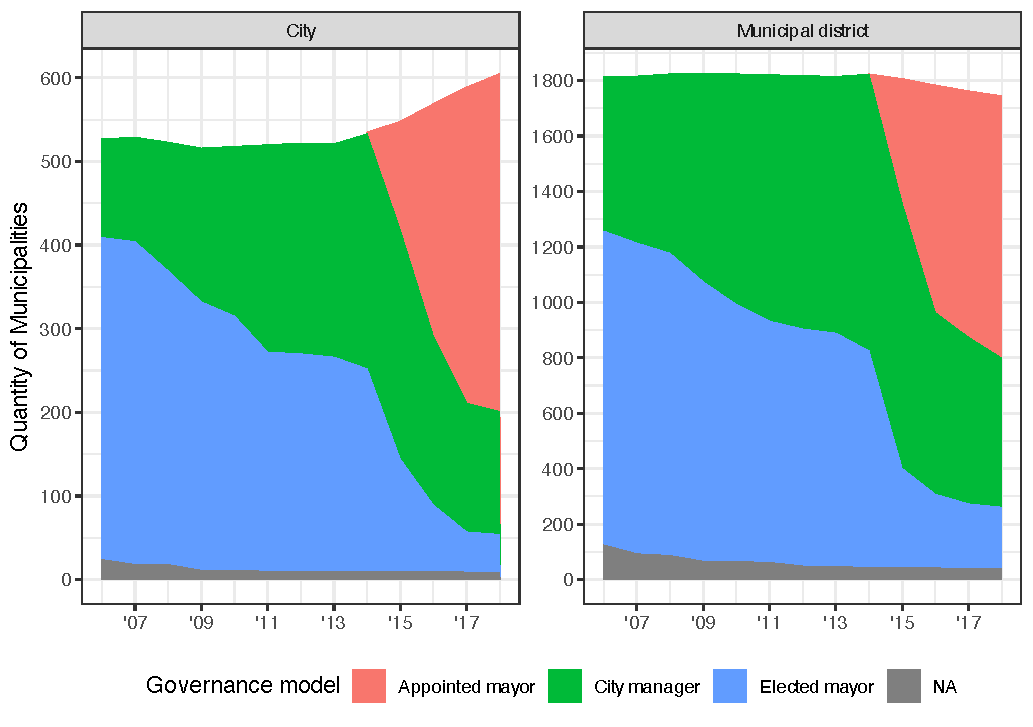
\includegraphics[width=0.8\textwidth]{Figures/model_by_year_plot.pdf}
\end{figure}



\newpage

\section{Empirical Methodology}





\begin{figure}[!htbp]\centering
    \caption{Distributions of Regions by a Share of Municipalities with Elected Mayors by Year}
    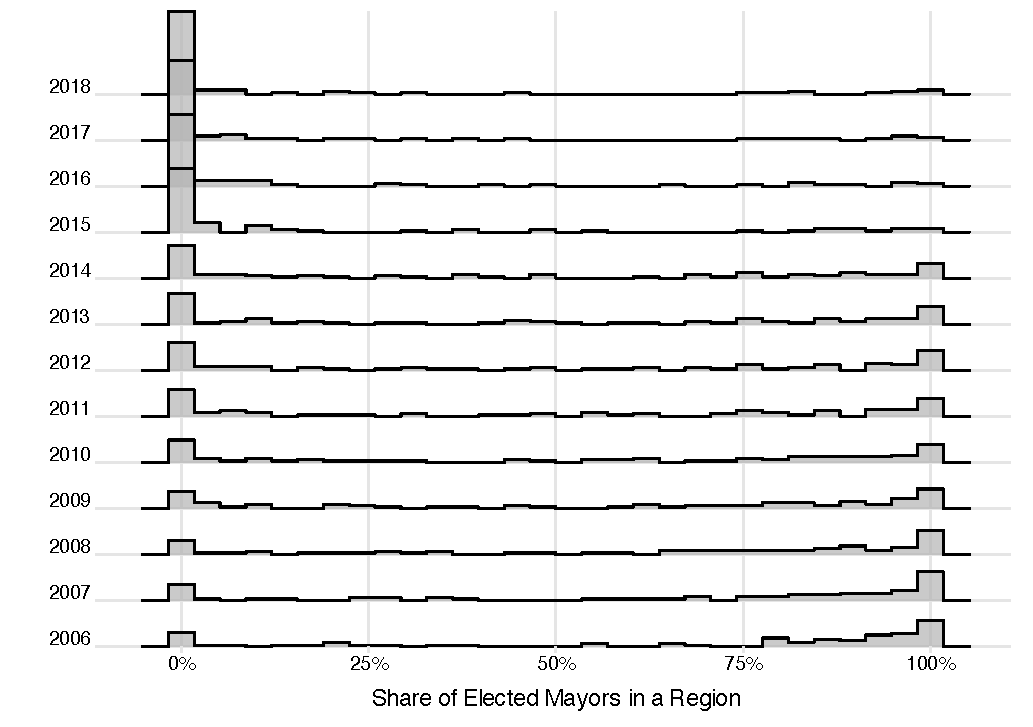
\includegraphics[width=\textwidth]{Figures/ridgeplot_models.pdf}
\end{figure}


\begin{figure}[!htbp]\centering
    \caption{Distribution of Regions by a Log of }
    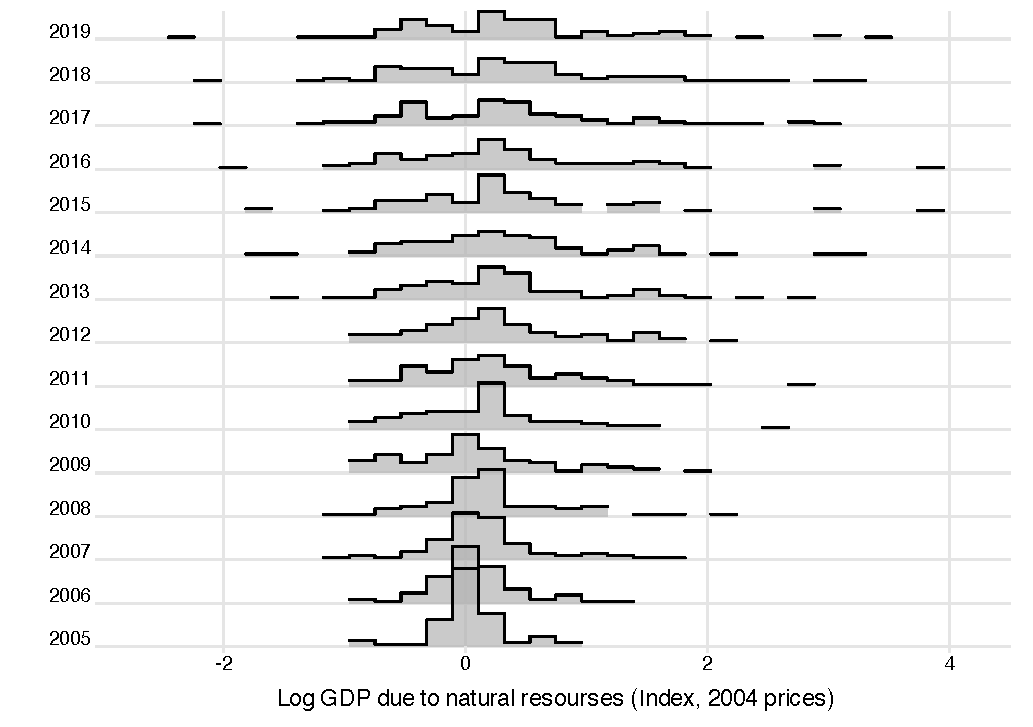
\includegraphics[width=\textwidth]{Figures/ridgeplot_resourse_extraction_gdp.pdf}
\end{figure}


\begin{table}[!htbp] \centering \footnotesize
\begin{threeparttable}
    \caption{Regional Economy Characteristic} 
    \label{} 
  \begin{tabular}{@{\extracolsep{5pt}}lccc} 
  \\[-1.8ex]\hline 
  \hline \\[-1.8ex] 
   & \multicolumn{3}{c}{\textit{Dependent variable:}  (\%) Share of municipalities with} \\ 
  \cline{2-4} 
  \\[-1.8ex] & Elected Mayors & City Managers & Appointed Mayors\\ 
  \\[-1.8ex] $\log$ of& (1) & (2) & (3)\\ 
  \hline \\[-1.8ex]
  $\textit{NR Extraction GRDP}$ & 4.129$^{**}$ & $-$0.827 & $-$3.302 \\ 
  & (2.030) & (2.255) & (2.077) \\ 
  & & & \\ 
  $\textit{Energy GDRP}$ & 10.986$^{**}$ & 12.675$^{**}$ & $-$23.661$^{***}$ \\ 
  & (4.736) & (5.264) & (4.847) \\ 
  & & & \\ 
 $\textit{Military GDRP}$ & 16.178 & $-$26.434$^{**}$ & 10.256 \\ 
  & (10.917) & (12.132) & (11.172) \\ 
  & & & \\ 
 $\textit{Manufacturing GDRP}$ & $-$14.219$^{***}$ & 6.358 & 7.861$^{**}$ \\ 
  & (3.873) & (4.304) & (3.963) \\ 
  & & & \\ 
 $\textit{Healthcare GDRP}$ & 22.616 & $-$23.343 & 0.726 \\ 
  & (14.965) & (16.631) & (15.316) \\ 
  & & & \\ 
 $\textit{Education GDRP}$ & $-$31.483$^{**}$ & $-$16.380 & 47.863$^{***}$ \\ 
  & (13.381) & (14.871) & (13.695) \\ 
  & & & \\ 
 $\textit{Construction GDRP}$ & $-$4.229 & 10.379$^{***}$ & $-$6.150$^{**}$ \\ 
  & (2.778) & (3.087) & (2.843) \\ 
  & & & \\ 
 $\textit{Aggriculture GDRP}$ & $-$2.059$^{**}$ & 2.463$^{**}$ & $-$0.404 \\ 
  & (1.005) & (1.117) & (1.028) \\ 
  & & & \\ 
 $\textit{Retail GDRP}$ & 1.778 & $-$5.690 & 3.912 \\ 
  & (6.703) & (7.449) & (6.860) \\ 
  & & & \\ 
 $\textit{Transport GDRP}$ & $-$19.925$^{***}$ & 13.362$^{**}$ & 6.563 \\ 
  & (5.801) & (6.447) & (5.937) \\ 
  & & & \\ 
 $\textit{Hospitality GDRP}$& 13.735$^{***}$ & $-$3.600 & $-$10.135$^{**}$ \\ 
  & (4.168) & (4.632) & (4.266) \\ 
  & & & \\ 
  $\textit{GRDP}$ & 8.941 & $-$4.574 & $-$4.368 \\ 
  & (9.540) & (10.601) & (9.763) \\ 
  & & & \\ 
 $\textit{population}$ & 103.047$^{**}$ & $-$33.273 & $-$69.774$^{*}$ \\ 
  & (41.190) & (45.774) & (42.156) \\ 
  & & & \\ 
  Time-Region Fixed Effects & Yes& Yes& Yes \\
  \hline \\[-1.8ex] 
  $N$ & 976 & 976 & 976 \\ 
  $n$ & 77& 77& 77\\
  $T$ & 4--13 & 4--13& 4--13\\
  F Statistic & 5.703$^{***}$ & 3.449$^{***}$ & 4.690$^{***}$ \\ 
  \hline 
  \hline 
  \end{tabular} 
  \begin{tablenotes}[flushleft]
    \item \textit{Notes:} Dependent variables are logs of GDRPs by  Double-clustering robust standard errors with HC3 influencial observations correction are in parenthesis \citep{Thompson2011,Cameron2011}. $^{*}\mathrm{p}<0.1$; $^{**}\mathrm{p}<0.05$; $^{***}\mathrm{p}<0.01$. Panel is unbalanced, $T=4$ for Crimea for which data is available from 2015 to 2018.
  \end{tablenotes}
\end{threeparttable}
  \end{table} 

\newpage 
\references


\appendix


\begin{sidewaystable}[!p] \centering \footnotesize
  \caption{Summary Statistics} 
  \label{} 
\begin{tabular}{@{\extracolsep{5pt}}lcccccccc} 
\\[-1.8ex]\hline 
\hline \\[-1.8ex] 
Statistic & \multicolumn{1}{c}{N} & \multicolumn{1}{c}{Min} & \multicolumn{1}{c}{Pctl(25)} & \multicolumn{1}{c}{Median} & \multicolumn{1}{c}{Mean} & \multicolumn{1}{c}{St. Dev.} & \multicolumn{1}{c}{Pctl(75)} & \multicolumn{1}{c}{Max} \\ 
\hline \\[-1.8ex] 
year & 986 & 2,006 & 2,009 & 2,012 & 2,012.049 & 3.738 & 2,015 & 2,018 \\ 
diff\_resourse\_gdp & 986 & 0.238 & 0.945 & 1.019 & 1.059 & 0.277 & 1.123 & 3.192 \\ 
resourse\_gdp & 986 & 0.112 & 0.792 & 1.147 & 1.810 & 3.045 & 1.717 & 50.653 \\ 
log\_resourse\_gdp & 986 & $-$2.193 & $-$0.233 & 0.137 & 0.230 & 0.730 & 0.541 & 3.925 \\ 
diff\_log\_resourse\_gdp & 985 & $-$1.435 & $-$0.056 & 0.019 & 0.028 & 0.244 & 0.116 & 1.161 \\ 
share\_city\_manager & 986 & 0.000 & 3.846 & 23.205 & 42.656 & 41.046 & 91.667 & 100.000 \\ 
share\_elected & 986 & 0.000 & 0.000 & 35.165 & 44.291 & 41.793 & 89.040 & 100.000 \\ 
share\_appointed & 986 & 0.000 & 0.000 & 0.000 & 13.053 & 31.381 & 0.000 & 100.000 \\ 
gdp\_pc & 976 & 43,797.200 & 146,519.100 & 227,995.200 & 355,664.500 & 591,670.100 & 350,496.800 & 7,296,374.000 \\ 
log\_gdp\_pc & 976 & 10.687 & 11.895 & 12.337 & 12.388 & 0.751 & 12.767 & 15.803 \\ 
log\_military\_gdp & 986 & $-$0.454 & 0.071 & 0.193 & 0.193 & 0.176 & 0.308 & 0.737 \\ 
log\_manufacturing\_gdp & 986 & $-$2.925 & 0.061 & 0.228 & 0.224 & 0.461 & 0.450 & 1.945 \\ 
log\_healthcare\_gdp & 986 & $-$0.429 & $-$0.050 & 0.024 & 0.047 & 0.157 & 0.133 & 0.742 \\ 
log\_energy\_gdp & 986 & $-$1.348 & $-$0.049 & 0.113 & 0.142 & 0.399 & 0.295 & 2.046 \\ 
log\_education\_gdp & 986 & $-$0.508 & $-$0.130 & $-$0.034 & $-$0.022 & 0.183 & 0.054 & 1.104 \\ 
log\_construction\_gdp & 986 & $-$2.334 & 0.192 & 0.483 & 0.448 & 0.476 & 0.738 & 1.725 \\ 
log\_aggriculture\_gdp & 986 & $-$0.240 & 3.566 & 6.095 & 5.904 & 2.988 & 8.305 & 20.234 \\ 
log\_retail\_gdp & 986 & $-$0.421 & 0.300 & 0.492 & 0.636 & 0.523 & 0.783 & 2.882 \\ 
log\_transport\_gdp & 986 & $-$0.245 & 0.182 & 0.346 & 0.533 & 0.547 & 0.667 & 3.075 \\ 
log\_hospitality\_gdp & 986 & $-$1.684 & 0.168 & 0.424 & 0.435 & 0.455 & 0.663 & 2.684 \\ 
gdp & 986 & 11,609.400 & 141,947.900 & 275,438.900 & 489,149.000 & 725,529.300 & 570,277.200 & 8,875,004.000 \\ 
log\_gdp & 986 & 9.360 & 11.863 & 12.526 & 12.514 & 1.088 & 13.254 & 15.999 \\ 
oil\_shock & 986 & $-$0.240 & $-$0.164 & 0.016 & $-$0.019 & 0.174 & 0.055 & 0.400 \\ 
population & 976 & 0.042 & 0.772 & 1.170 & 1.585 & 1.285 & 2.331 & 7.552 \\ 
\hline \\[-1.8ex] 
\end{tabular} 
\end{sidewaystable} 

\end{document}